\documentclass{beamer}
%%% ========== Package setup ==========
\usepackage{xeCJK}      % Chinese words package
\usepackage{fontspec}   % Word fonts package
\usepackage{listings}   % Wrap Figure or table package
\usepackage{wrapfig}    % Multicolumn package
\usepackage{multicol}   % Multicolumn package
\usepackage{pdflscape}  % Landscpae package
\usepackage{tikz}       % TikZ picture package(Docs: https://ftp.ntou.edu.tw/ctan/graphics/pgf/base/doc/pgfmanual.pdf)
\usepackage[outline]{contour} % glow around text
\usepackage{amsmath}
\usepackage{mathtools}

%%% ========== Slide setting ==========
%% Slide theme setup
\usetheme{CambridgeUS}
\usecolortheme{wolverine}

%% Setup chinese words encoder
\XeTeXlinebreaklocale "zh"
\XeTeXlinebreakskip = 0pt plus 1pt

%% More word fonts
\setmainfont{Times New Roman}
\renewcommand{\familydefault}{\rmdefault}
\setCJKmainfont{標楷體}

% Setting for figure and table numbering
\setbeamertemplate{caption}[numbered]

% TikZ setting
\usetikzlibrary{positioning}
\usetikzlibrary{calc}
\usetikzlibrary{arrows.meta}

%%% ========== Title setup ==========
\date{July 04, 2022}
\title{Meeting}
\author{Po Hsun Wu}

%%% ========== Document ==========
\begin{document}
    \maketitle

    \section*{Progress report}
    \begin{frame}
        \frametitle{\secname}

        \begin{itemize}
            \item Studying Q-larning algromn.
            $$\max_{\theta} Q(x(t), u(t))$$
            Iteration equation:
            $$Q^{(n+1)}(x_t, u_t) = Q^{(n)}(x_t, u_t) + \alpha(r_t + \gamma\max_{u}Q^{(n)}(x_{t+1}, u))$$

        \end{itemize}

    \end{frame}

    \begin{frame}
        \frametitle{\secname}

        \begin{figure}
            \begin{multicols}{2}
                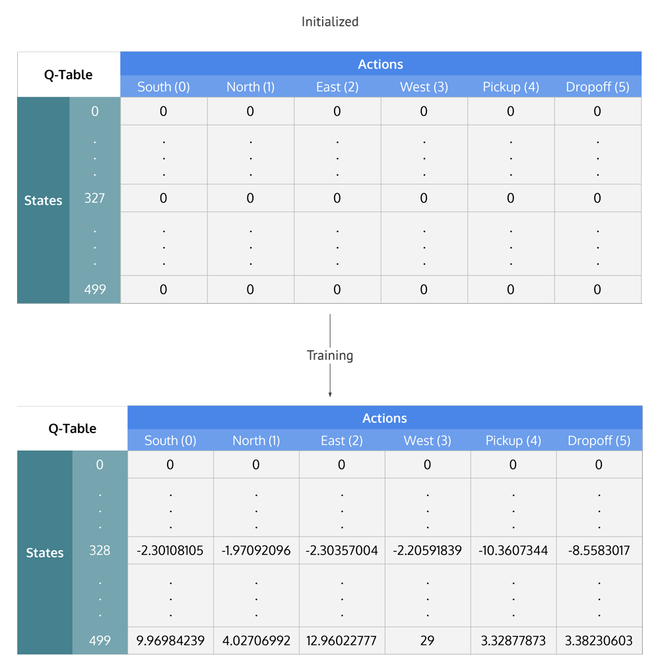
\includegraphics[scale=.25]{./Figs/Qtable.png}
                \caption{Q-table}

                \columnbreak
                %%% ==================== QLearning flow chart with NN ====================
% The figure of Q-learning flow chart with neural network
% Author: Wu, Po Hsun
% Date: June 08, 2022
%
\tikzstyle{circlenode}=[circle, draw=black, thick, minimum size=1mm]
\tikzstyle{squarednode}=[rectangle, draw=black, thick, minimum size=0mm, font=\footnotesize]

\begin{tikzpicture}[
    ->, >={latex},
    node distance=0.5cm,
    every state/.style={thick}
    ]
    % ---------- Nodes ----------
    \node[squarednode]  (initialQtable)     []                          {Initialize Q-table \& NN};
    \node[squarednode]  (chooseAction)      [below=of initialQtable]    {Choose a action from NN};
    \node[squarednode]  (obtainState)       [below=of chooseAction]     {Obtain the state from the environment};
    \node[squarednode]  (measureReward)     [below=of obtainState]      {Measure the reward};
    \node[squarednode]  (updateQtable)      [below=of measureReward]    {Update Q-table};
    \node[squarednode]  (trainNN)           [below=of updateQtable]     {Train the NN};

    % ---------- Lines ----------
    \draw[] (initialQtable.south) -- (chooseAction.north);
    \draw[] (chooseAction.south) -- (obtainState.north);
    \draw[] (obtainState.south) -- (measureReward.north);
    \draw[] (measureReward.south) -- (updateQtable.north);
    \draw[] (updateQtable.south) -- (trainNN.north);
    \draw[] (trainNN.south) |- ++(-3,-0.5) |- (chooseAction.west);

\end{tikzpicture}
                \caption{Flow chart of Q-learning}
            \end{multicols}
        \end{figure}

    \end{frame}

    \begin{frame}
        \frametitle{\secname}

        \begin{itemize}
            \item Checking the environment.
        \end{itemize}
        \begin{figure}
            \begin{multicols*}{2}
                \centering
                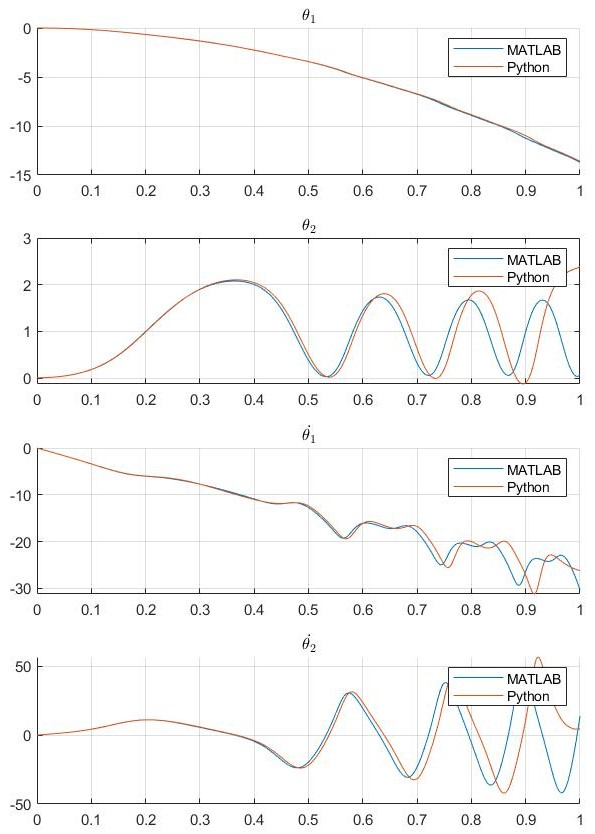
\includegraphics[scale=.25]{./Figs/state.jpg}
                \caption{State}

                \columnbreak
                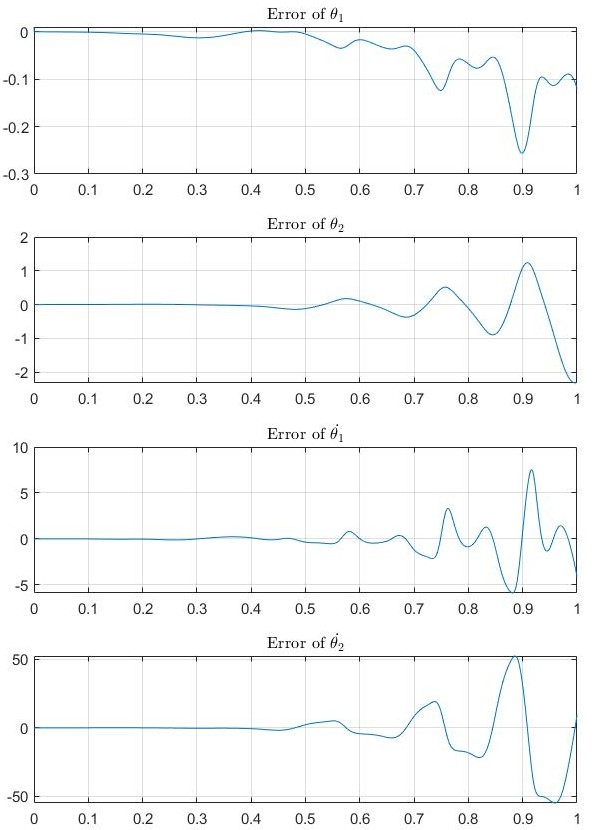
\includegraphics[scale=.25]{./Figs/error.jpg}
                \caption{Error}
            \end{multicols*}
        \end{figure}

    \end{frame}
\end{document}